\documentclass[tikz,border=6pt]{standalone}
\usepackage[T1]{fontenc}
\usepackage[utf8]{inputenc}
\usepackage{helvet}
\renewcommand{\familydefault}{\sfdefault}
\usepackage{siunitx}
\usetikzlibrary{arrows.meta,calc,positioning,shapes.geometric}

\definecolor{Navy}{HTML}{0B1F33}
\definecolor{Ink}{HTML}{183247}
\definecolor{Slate}{HTML}{5D7182}
\definecolor{Line}{HTML}{C7D5DE}
\definecolor{Panel}{HTML}{F5F8FA}
\definecolor{Blue}{HTML}{2678B8}
\definecolor{BlueLight}{HTML}{DCECF7}
\definecolor{Orange}{HTML}{E88932}
\definecolor{OrangeLight}{HTML}{FCE9D6}
\definecolor{Teal}{HTML}{00A7A0}
\definecolor{TealLight}{HTML}{DDF4F1}
\definecolor{Green}{HTML}{5B9E62}
\definecolor{Red}{HTML}{C94D4D}
\definecolor{Grey}{HTML}{7D8C97}
\definecolor{GreyLight}{HTML}{E8EEF2}

\tikzset{
  panel/.style={rounded corners=2mm, draw=Line, line width=0.7pt, fill=Panel},
  box/.style={rounded corners=1.2mm, draw=Line, line width=0.7pt, fill=white,
    align=center, inner sep=2.0mm, font=\sffamily\scriptsize},
  flow/.style={-{Latex[length=2.5mm,width=1.6mm]}, line width=1.15pt},
  waterrev/.style={{Latex[length=2.7mm,width=1.8mm]}-{Latex[length=2.7mm,width=1.8mm]},
    line width=1.35pt, Teal},
  dim/.style={{Bar[width=4pt]}-{Bar[width=4pt]}, line width=0.55pt, Slate},
  leader/.style={line width=0.55pt, Slate}
}

\begin{document}
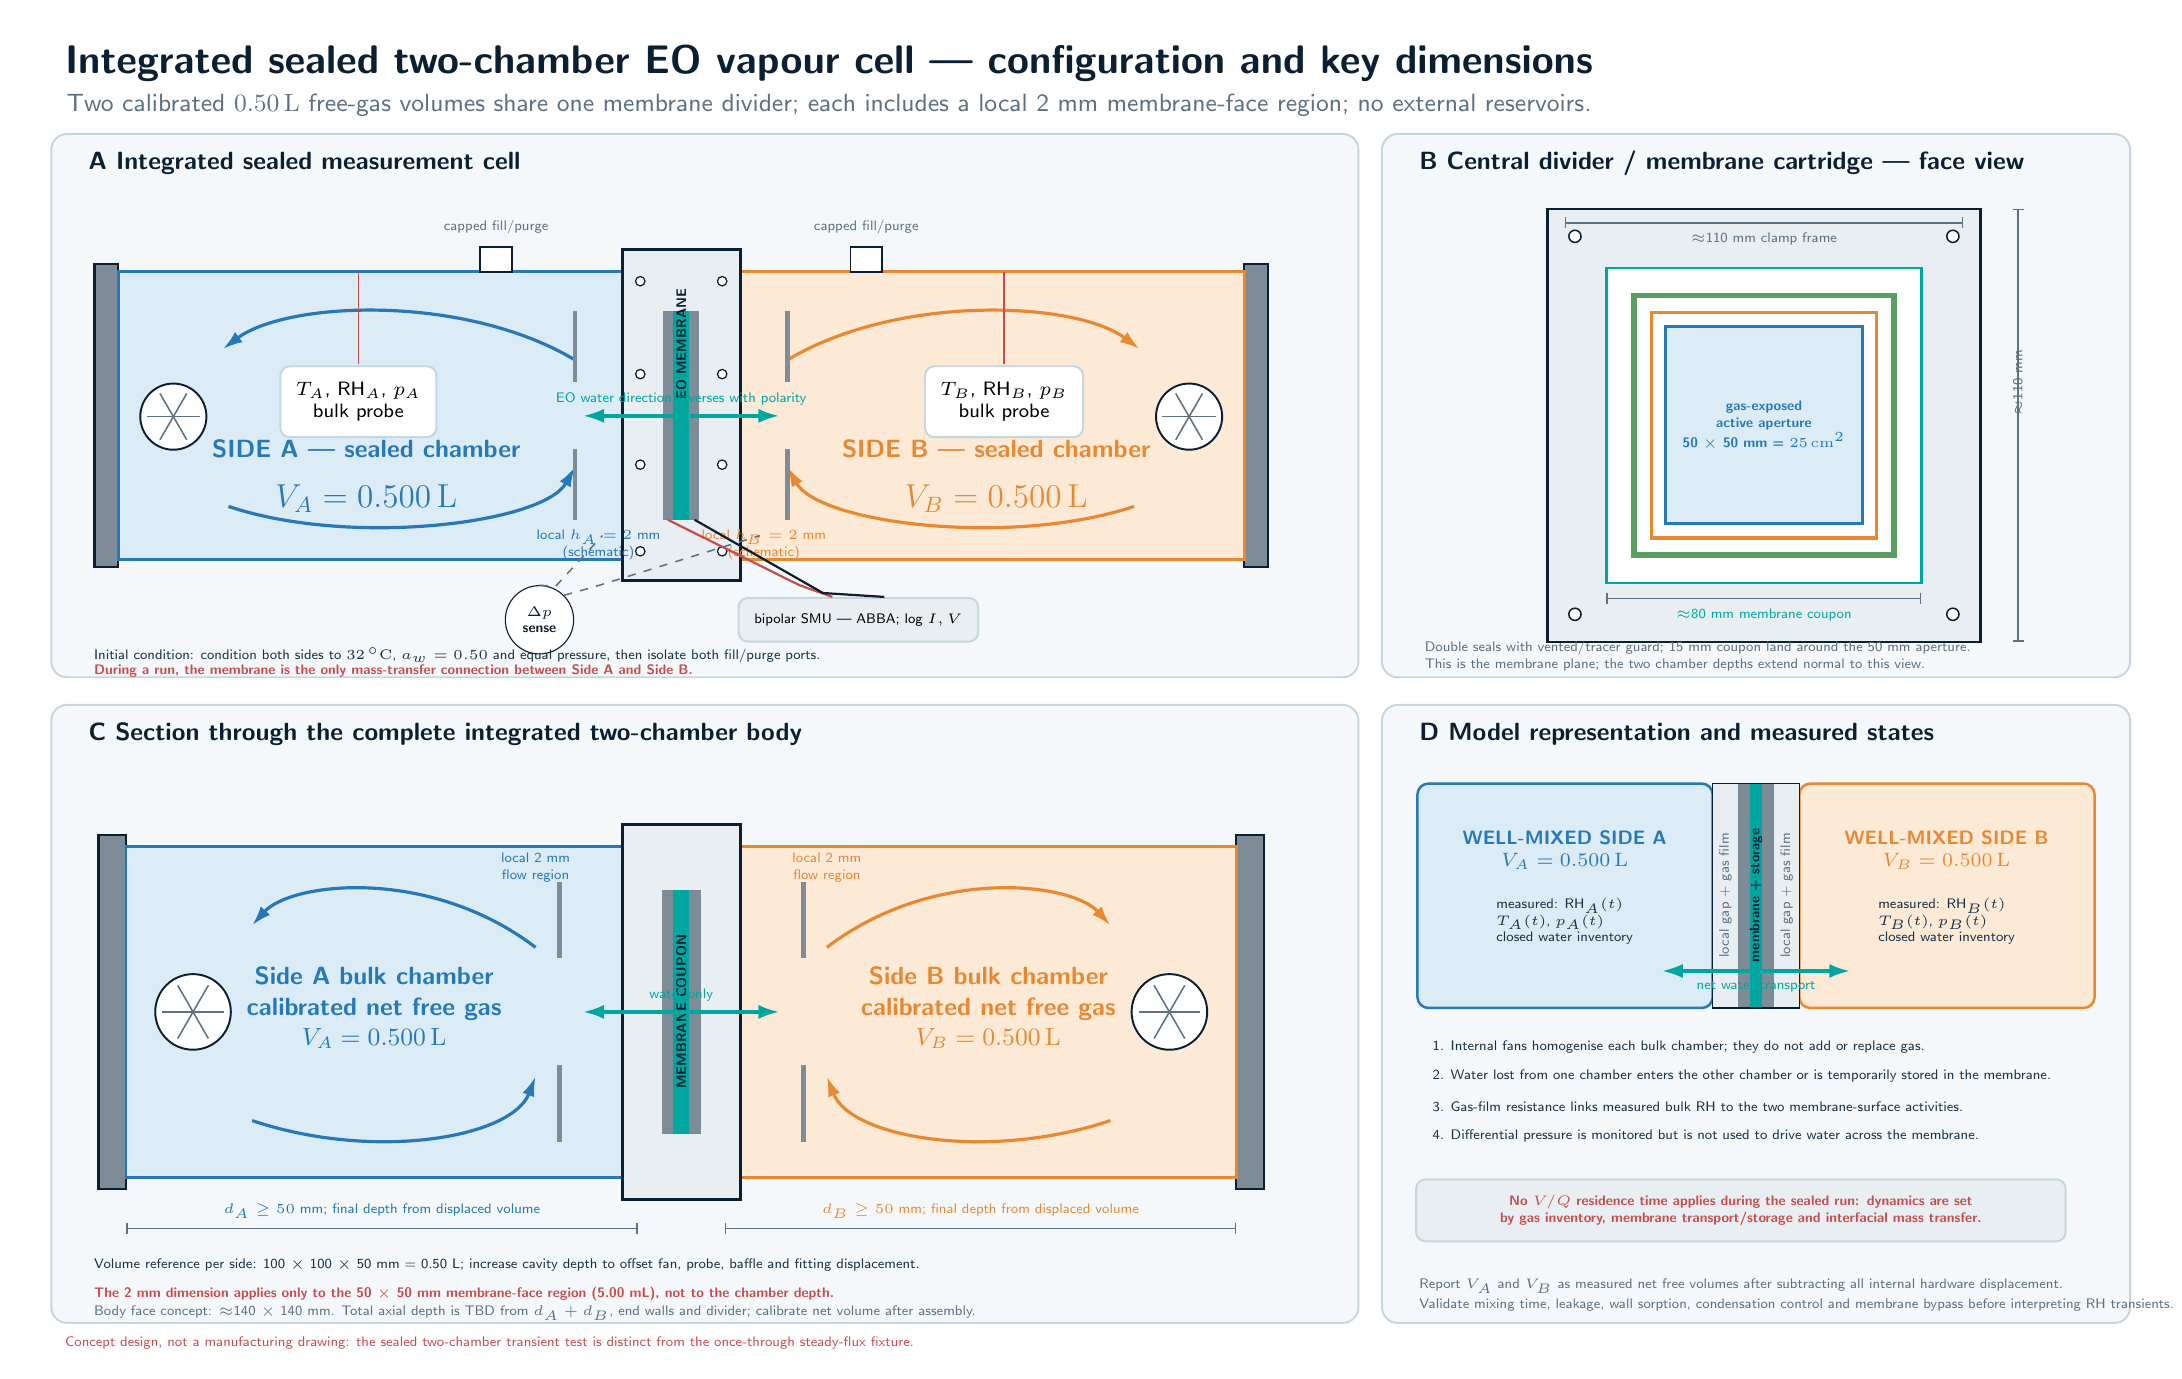
\begin{tikzpicture}[x=1cm,y=1cm]
  \path[use as bounding box] (0,0) rectangle (27,16.8);

  % Title
  \node[anchor=west, font=\sffamily\bfseries\Large, text=Navy]
    at (0.35,16.35) {Integrated sealed two-chamber EO vapour cell --- configuration and key dimensions};
  \node[anchor=west, font=\sffamily\small, text=Slate]
    at (0.37,15.82) {Two calibrated \SI{0.50}{L} free-gas volumes share one membrane divider; each includes a local 2 mm membrane-face region; no external reservoirs.};

  % ---------------------------------------------------------------------------
  % Panel A: integrated sealed cell
  % ---------------------------------------------------------------------------
  \draw[panel] (0.3,8.55) rectangle (16.9,15.45);
  \node[anchor=west, font=\sffamily\bfseries\small, text=Navy]
    at (0.65,15.08) {A  Integrated sealed measurement cell};

  % Outer body and chambers
  \fill[Grey] (0.85,9.95) rectangle (1.15,13.80);
  \fill[Grey] (15.45,9.95) rectangle (15.75,13.80);
  \draw[Navy, line width=0.8pt] (0.85,9.95) rectangle (1.15,13.80);
  \draw[Navy, line width=0.8pt] (15.45,9.95) rectangle (15.75,13.80);
  \fill[BlueLight] (1.15,10.05) rectangle (7.75,13.70);
  \fill[OrangeLight] (8.85,10.05) rectangle (15.45,13.70);
  \draw[Blue, line width=1.0pt] (1.15,10.05) rectangle (7.75,13.70);
  \draw[Orange, line width=1.0pt] (8.85,10.05) rectangle (15.45,13.70);

  % Central cartridge and membrane stack
  \fill[GreyLight] (7.55,9.78) rectangle (9.05,13.98);
  \draw[Navy, line width=1.0pt] (7.55,9.78) rectangle (9.05,13.98);
  \fill[Grey] (8.07,10.55) rectangle (8.20,13.20);
  \fill[Teal] (8.20,10.55) rectangle (8.40,13.20);
  \fill[Grey] (8.40,10.55) rectangle (8.53,13.20);
  \foreach \yy in {10.15,11.25,12.40,13.58} {
    \fill[white] (7.78,\yy) circle (1.7pt);
    \draw[Navy, line width=0.45pt] (7.78,\yy) circle (1.7pt);
    \fill[white] (8.82,\yy) circle (1.7pt);
    \draw[Navy, line width=0.45pt] (8.82,\yy) circle (1.7pt);
  }
  \node[rotate=90, font=\sffamily\bfseries\tiny, text=Navy] at (8.30,12.78) {EO MEMBRANE};

  % Internal fans and mixing arrows
  \draw[Navy, line width=0.7pt, fill=white] (1.85,11.86) circle (0.42);
  \draw[Navy, line width=0.7pt, fill=white] (14.75,11.86) circle (0.42);
  \foreach \a in {0,60,...,300} {
    \draw[Slate, line width=0.55pt] (1.85,11.86) -- ++(\a:0.34);
    \draw[Slate, line width=0.55pt] (14.75,11.86) -- ++(\a:0.34);
  }
  \draw[flow, Blue] (2.55,10.72) .. controls (4.10,10.20) and (6.55,10.50) .. (6.95,11.22);
  \draw[flow, Blue] (6.95,12.58) .. controls (5.55,13.42) and (3.30,13.33) .. (2.48,12.72);
  \draw[flow, Orange] (14.05,10.72) .. controls (12.50,10.20) and (10.05,10.50) .. (9.65,11.22);
  \draw[flow, Orange] (9.65,12.58) .. controls (11.05,13.42) and (13.30,13.33) .. (14.12,12.72);
  \draw[Grey, line width=1.6pt] (6.95,10.55) -- (6.95,11.45);
  \draw[Grey, line width=1.6pt] (6.95,12.30) -- (6.95,13.20);
  \draw[Grey, line width=1.6pt] (9.65,10.55) -- (9.65,11.45);
  \draw[Grey, line width=1.6pt] (9.65,12.30) -- (9.65,13.20);
  \node[align=center, font=\sffamily\tiny, text=Blue] at (7.25,10.23)
    {local $h_A=2$ mm\\(schematic)};
  \node[align=center, font=\sffamily\tiny, text=Orange] at (9.35,10.23)
    {local $h_B=2$ mm\\(schematic)};

  % Sensors and sealed conditioning ports
  \node[box, minimum width=1.65cm, minimum height=0.82cm, fill=white]
    (sensA) at (4.20,12.05) {$T_A$, RH$_A$, $p_A$\\bulk probe};
  \node[box, minimum width=1.65cm, minimum height=0.82cm, fill=white]
    (sensB) at (12.40,12.05) {$T_B$, RH$_B$, $p_B$\\bulk probe};
  \draw[Red, line width=0.6pt] (4.20,13.70) -- (4.20,12.53);
  \draw[Red, line width=0.6pt] (12.40,13.70) -- (12.40,12.53);
  \draw[Navy, line width=0.7pt, fill=white] (5.75,13.70) rectangle (6.15,14.02);
  \draw[Navy, line width=0.7pt, fill=white] (10.45,13.70) rectangle (10.85,14.02);
  \node[anchor=south, font=\sffamily\tiny, text=Slate] at (5.95,14.06) {capped fill/purge};
  \node[anchor=south, font=\sffamily\tiny, text=Slate] at (10.65,14.06) {capped fill/purge};

  % Labels, water direction and electrical drive
  \node[font=\sffamily\bfseries\small, text=Blue] at (4.30,11.45) {SIDE A --- sealed chamber};
  \node[font=\sffamily\bfseries\large, text=Blue] at (4.30,10.82) {$V_A=\SI{0.500}{L}$};
  \node[font=\sffamily\bfseries\small, text=Orange] at (12.30,11.45) {SIDE B --- sealed chamber};
  \node[font=\sffamily\bfseries\large, text=Orange] at (12.30,10.82) {$V_B=\SI{0.500}{L}$};
  \draw[waterrev] (7.05,11.87) -- node[above, font=\sffamily\tiny, text=Teal]
    {EO water direction reverses with polarity} (9.55,11.87);

  \node[box, minimum width=1.95cm, minimum height=0.52cm, fill=GreyLight,
    font=\sffamily\tiny] (smu) at (10.55,9.28) {bipolar SMU --- ABBA; log $I,V$};
  \draw[Red, line width=0.8pt] ($(smu.north)+(-0.33,0)$) -- (9.80,9.72) -- (8.13,10.55);
  \draw[Navy, line width=0.8pt] ($(smu.north)+(0.33,0)$) -- (10.10,9.62) -- (8.47,10.55);
  \node[circle, draw=Navy, fill=white, minimum size=0.66cm, align=center,
    font=\sffamily\bfseries\tiny, text=Navy] (dp) at (6.50,9.28) {$\Delta p$\\sense};
  \draw[dashed, leader] (dp.north) -- (6.70,9.70) -- (7.30,10.35);
  \draw[dashed, leader] (dp.north east) -- (7.20,9.70) -- (9.30,10.35);

  \node[anchor=west, font=\sffamily\tiny, text=Ink]
    at (0.72,8.83) {Initial condition: condition both sides to \SI{32}{\celsius}, $a_w=0.50$ and equal pressure, then isolate both fill/purge ports.};
  \node[anchor=west, font=\sffamily\bfseries\tiny, text=Red]
    at (0.72,8.63) {During a run, the membrane is the only mass-transfer connection between Side A and Side B.};

  % ---------------------------------------------------------------------------
  % Panel B: membrane cartridge face view
  % ---------------------------------------------------------------------------
  \draw[panel] (17.2,8.55) rectangle (26.7,15.45);
  \node[anchor=west, font=\sffamily\bfseries\small, text=Navy]
    at (17.55,15.08) {B  Central divider / membrane cartridge --- face view};

  \fill[GreyLight] (19.30,9.00) rectangle (24.80,14.50);
  \draw[Navy, line width=0.9pt] (19.30,9.00) rectangle (24.80,14.50);
  \fill[white] (20.05,9.75) rectangle (24.05,13.75);
  \draw[Teal, line width=0.8pt] (20.05,9.75) rectangle (24.05,13.75);
  \draw[Green, line width=2.0pt] (20.40,10.10) rectangle (23.70,13.40);
  \draw[Orange, line width=1.2pt] (20.62,10.32) rectangle (23.48,13.18);
  \draw[Green, line width=1.5pt] (20.82,10.52) rectangle (23.28,12.98);
  \fill[BlueLight] (20.80,10.50) rectangle (23.30,13.00);
  \draw[Blue, line width=1.0pt] (20.80,10.50) rectangle (23.30,13.00);
  \node[align=center, font=\sffamily\bfseries\tiny, text=Blue] at (22.05,11.75)
    {gas-exposed\\active aperture\\50 $\times$ 50 mm = \SI{25}{cm^2}};
  \foreach \x/\y in {19.65/9.35,24.45/9.35,19.65/14.15,24.45/14.15} {
    \fill[white] (\x,\y) circle (2.2pt);
    \draw[Navy, line width=0.55pt] (\x,\y) circle (2.2pt);
  }
  \draw[dim] (19.52,14.32) -- node[below, font=\sffamily\tiny, text=Slate]
    {$\approx$110 mm clamp frame} (24.58,14.32);
  \draw[dim] (25.28,9.00) -- node[right, rotate=90, font=\sffamily\tiny, text=Slate]
    {$\approx$110 mm} (25.28,14.50);
  \draw[dim] (20.05,9.55) -- node[below, font=\sffamily\tiny, text=Teal]
    {$\approx$80 mm membrane coupon} (24.05,9.55);
  \node[anchor=west, font=\sffamily\tiny, text=Slate] at (17.62,8.92)
    {Double seals with vented/tracer guard; 15 mm coupon land around the 50 mm aperture.};
  \node[anchor=west, font=\sffamily\tiny, text=Slate] at (17.62,8.70)
    {This is the membrane plane; the two chamber depths extend normal to this view.};

  % ---------------------------------------------------------------------------
  % Panel C: full integrated cross-section
  % ---------------------------------------------------------------------------
  \draw[panel] (0.3,0.35) rectangle (16.9,8.20);
  \node[anchor=west, font=\sffamily\bfseries\small, text=Navy]
    at (0.65,7.82) {C  Section through the complete integrated two-chamber body};

  \fill[Grey] (0.90,2.05) rectangle (1.25,6.55);
  \fill[Grey] (15.35,2.05) rectangle (15.70,6.55);
  \draw[Navy, line width=0.8pt] (0.90,2.05) rectangle (1.25,6.55);
  \draw[Navy, line width=0.8pt] (15.35,2.05) rectangle (15.70,6.55);
  \fill[BlueLight] (1.25,2.20) rectangle (7.75,6.40);
  \fill[OrangeLight] (8.85,2.20) rectangle (15.35,6.40);
  \draw[Blue, line width=1.0pt] (1.25,2.20) rectangle (7.75,6.40);
  \draw[Orange, line width=1.0pt] (8.85,2.20) rectangle (15.35,6.40);

  \fill[GreyLight] (7.55,1.92) rectangle (9.05,6.68);
  \draw[Navy, line width=1.0pt] (7.55,1.92) rectangle (9.05,6.68);
  \fill[Grey] (8.05,2.75) rectangle (8.20,5.85);
  \fill[Teal] (8.20,2.75) rectangle (8.40,5.85);
  \fill[Grey] (8.40,2.75) rectangle (8.55,5.85);
  \node[rotate=90, font=\sffamily\bfseries\tiny, text=Navy] at (8.30,4.30) {MEMBRANE COUPON};

  % Mixing hardware shown as displaced internal volume
  \draw[Navy, line width=0.7pt, fill=white] (2.10,4.30) circle (0.48);
  \draw[Navy, line width=0.7pt, fill=white] (14.50,4.30) circle (0.48);
  \foreach \a in {0,60,...,300} {
    \draw[Slate, line width=0.55pt] (2.10,4.30) -- ++(\a:0.39);
    \draw[Slate, line width=0.55pt] (14.50,4.30) -- ++(\a:0.39);
  }
  \draw[Grey, line width=1.8pt] (6.75,2.65) -- (6.75,3.62);
  \draw[Grey, line width=1.8pt] (6.75,4.98) -- (6.75,5.95);
  \draw[Grey, line width=1.8pt] (9.85,2.65) -- (9.85,3.62);
  \draw[Grey, line width=1.8pt] (9.85,4.98) -- (9.85,5.95);
  \draw[flow, Blue] (2.85,2.92) .. controls (4.40,2.40) and (6.15,2.70) .. (6.45,3.48);
  \draw[flow, Blue] (6.45,5.12) .. controls (5.10,6.15) and (3.35,5.95) .. (2.85,5.40);
  \draw[flow, Orange] (13.75,2.92) .. controls (12.20,2.40) and (10.45,2.70) .. (10.15,3.48);
  \draw[flow, Orange] (10.15,5.12) .. controls (11.50,6.15) and (13.25,5.95) .. (13.75,5.40);

  \node[align=center, font=\sffamily\bfseries\small, text=Blue] at (4.40,4.35)
    {Side A bulk chamber\\calibrated net free gas\\$V_A=\SI{0.500}{L}$};
  \node[align=center, font=\sffamily\bfseries\small, text=Orange] at (12.20,4.35)
    {Side B bulk chamber\\calibrated net free gas\\$V_B=\SI{0.500}{L}$};
  \draw[waterrev] (7.05,4.30) -- node[above, font=\sffamily\tiny, text=Teal]
    {water only} (9.55,4.30);

  \node[align=center, font=\sffamily\tiny, text=Blue] at (6.45,6.13)
    {local 2 mm\\flow region};
  \node[align=center, font=\sffamily\tiny, text=Orange] at (10.15,6.13)
    {local 2 mm\\flow region};

  \draw[dim] (1.25,1.55) -- node[above, font=\sffamily\tiny, text=Blue]
    {$d_A\geq50$ mm; final depth from displaced volume} (7.75,1.55);
  \draw[dim] (8.85,1.55) -- node[above, font=\sffamily\tiny, text=Orange]
    {$d_B\geq50$ mm; final depth from displaced volume} (15.35,1.55);
  \node[anchor=west, font=\sffamily\tiny, text=Ink] at (0.72,1.08)
    {Volume reference per side: 100 $\times$ 100 $\times$ 50 mm = 0.50 L; increase cavity depth to offset fan, probe, baffle and fitting displacement.};
  \node[anchor=west, font=\sffamily\bfseries\tiny, text=Red] at (0.72,0.72)
    {The 2 mm dimension applies only to the 50 $\times$ 50 mm membrane-face region (5.00 mL), not to the chamber depth.};
  \node[anchor=west, font=\sffamily\tiny, text=Slate] at (0.72,0.47)
    {Body face concept: $\approx$140 $\times$ 140 mm. Total axial depth is TBD from $d_A+d_B$, end walls and divider; calibrate net volume after assembly.};

  % ---------------------------------------------------------------------------
  % Panel D: model representation
  % ---------------------------------------------------------------------------
  \draw[panel] (17.2,0.35) rectangle (26.7,8.20);
  \node[anchor=west, font=\sffamily\bfseries\small, text=Navy]
    at (17.55,7.82) {D  Model representation and measured states};

  \draw[rounded corners=1.4mm, draw=Blue, line width=0.9pt, fill=BlueLight]
    (17.65,4.35) rectangle (21.40,7.20);
  \draw[rounded corners=1.4mm, draw=Orange, line width=0.9pt, fill=OrangeLight]
    (22.50,4.35) rectangle (26.25,7.20);
  \fill[GreyLight] (21.40,4.35) rectangle (21.72,7.20);
  \fill[Grey] (21.72,4.35) rectangle (21.87,7.20);
  \fill[Teal] (21.87,4.35) rectangle (22.03,7.20);
  \fill[Grey] (22.03,4.35) rectangle (22.18,7.20);
  \fill[GreyLight] (22.18,4.35) rectangle (22.50,7.20);
  \draw[Navy, line width=0.5pt] (21.40,4.35) rectangle (22.50,7.20);

  \node[align=center, font=\sffamily\bfseries\scriptsize, text=Blue] at (19.52,6.35)
    {WELL-MIXED SIDE A\\$V_A=\SI{0.500}{L}$};
  \node[align=left, font=\sffamily\tiny, text=Ink] at (19.52,5.45)
    {measured: RH$_A(t)$\\$T_A(t)$, $p_A(t)$\\closed water inventory};
  \node[align=center, font=\sffamily\bfseries\scriptsize, text=Orange] at (24.37,6.35)
    {WELL-MIXED SIDE B\\$V_B=\SI{0.500}{L}$};
  \node[align=left, font=\sffamily\tiny, text=Ink] at (24.37,5.45)
    {measured: RH$_B(t)$\\$T_B(t)$, $p_B(t)$\\closed water inventory};
  \node[rotate=90, font=\sffamily\tiny, text=Slate] at (21.56,5.78) {local gap + gas film};
  \node[rotate=90, font=\sffamily\tiny, text=Slate] at (22.34,5.78) {local gap + gas film};
  \node[rotate=90, font=\sffamily\bfseries\tiny, text=Navy] at (21.95,5.78) {membrane + storage};
  \draw[waterrev] (20.75,4.82) -- node[below, font=\sffamily\tiny, text=Teal]
    {net water transport} (23.15,4.82);

  \node[anchor=west, font=\sffamily\tiny, text=Ink] at (17.72,3.86)
    {1. Internal fans homogenise each bulk chamber; they do not add or replace gas.};
  \node[anchor=west, font=\sffamily\tiny, text=Ink] at (17.72,3.48)
    {2. Water lost from one chamber enters the other chamber or is temporarily stored in the membrane.};
  \node[anchor=west, font=\sffamily\tiny, text=Ink] at (17.72,3.10)
    {3. Gas-film resistance links measured bulk RH to the two membrane-surface activities.};
  \node[anchor=west, font=\sffamily\tiny, text=Ink] at (17.72,2.72)
    {4. Differential pressure is monitored but is not used to drive water across the membrane.};

  \node[box, anchor=west, minimum width=8.25cm, minimum height=0.78cm,
    text width=7.75cm, fill=GreyLight, font=\sffamily\bfseries\tiny, text=Red]
    at (17.62,1.78) {No $V/Q$ residence time applies during the sealed run: dynamics are set by gas inventory, membrane transport/storage and interfacial mass transfer.};
  \node[anchor=west, font=\sffamily\tiny, text=Slate] at (17.55,0.82)
    {Report $V_A$ and $V_B$ as measured net free volumes after subtracting all internal hardware displacement.};
  \node[anchor=west, font=\sffamily\tiny, text=Slate] at (17.55,0.58)
    {Validate mixing time, leakage, wall sorption, condensation control and membrane bypass before interpreting RH transients.};

  \node[anchor=west, font=\sffamily\tiny, text=Red]
    at (0.35,0.10) {Concept design, not a manufacturing drawing: the sealed two-chamber transient test is distinct from the once-through steady-flux fixture.};

\end{tikzpicture}
\end{document}
